\documentclass[a4paper,12pt,oneside]{article}
\usepackage[english]{babel} % für die deutsche Sprache
\usepackage[utf8]{inputenc} % Für die direkte Eingabe von Umlauten im Editor u.a.
\usepackage[T1]{fontenc}
\usepackage[dvipsnames]{xcolor}
\usepackage{listings}
\usepackage{fancyhdr} % Für Kopf- und Fußzeilen
\usepackage{graphicx} % Zum Laden von Graphiken
\usepackage{setspace} % Paket zum Setzen des Zeilenabstandes
\usepackage{helvet}
\usepackage{mathptmx}
\usepackage{float}
\usepackage{caption}
\usepackage{ragged2e}
\usepackage{gensymb}
\usepackage{amsmath}
\usepackage{makecell}
\usepackage{amsmath}
\usepackage[colorlinks,pdfpagelabels,pdfstartview=FitH,
bookmarksopen=true,bookmarksnumbered=true,linkcolor=black,
plainpages=false,hypertexnames=false,citecolor=black]{hyperref} % Für Verlinkungen

%%--------------
%\usepackage[normalem]{ulem} % Für das Unterstreichen von Text z.B. mit \uline{}
\usepackage[left=2cm,right=2cm,top=1.5cm,bottom=1cm,
textheight=245mm,textwidth=160mm,includeheadfoot,headsep=1cm,
footskip=1cm,headheight=14.599pt]{geometry} % Einrichtung der Seite 

\onehalfspacing % Zeilenabstand auf 1,5-zeilig setzen
\setlength{\parindent}{0pt} % Einrückung nach Zeilenabstand unterdrücken

  \fancypagestyle{TOC}{% Seitenlayout Inhaltsverzeichnich, Abbildungsverzeichnis
  \fancyhf{} % clear all header and footer fields
  \fancyfoot[R]{\thepage} 
  \renewcommand{\headrulewidth}{0pt}
  \renewcommand{\footrulewidth}{0pt}}

\lstset{
  basicstyle=\color{darkgray},
%  backgroundcolor=\color{darkgray},
  showstringspaces=false,
  commentstyle=\color{ForestGreen},
  breaklines=true,
  postbreak=\mbox{\textcolor{red}{$\hookrightarrow$}\space},
  columns=fullflexible,
  keywordstyle=\color{darkgray},
  language=bash,
  emph={\$},
  emphstyle={\color{blue}\bfseries}
}
  
\lstset{literate=%
    {Ö}{{\"O}}1
    {Ä}{{\"A}}1
    {Ü}{{\"U}}1
    {ß}{{\ss}}1
    {ü}{{\"u}}1
    {ä}{{\"a}}1
    {ö}{{\"o}}1
    {-}{{-}}1
    {-->}{{ $\Rightarrow$ }}1
    {>>}{{\glqq}}1
    {<<}{{\grqq}}1
}

\begin{document}

\pagestyle{empty}
\pagenumbering{roman}
\begin{titlepage}
	
\includegraphics[scale=1.00]{sources/logo_TH-Koeln_CMYK_22pt-eps-converted-to.pdf}\\
	\begin{center}
		\large
		University of Applied Sciences Cologne\\
		Special Aspects of Mobile Autonomous Systems\\
		
\includegraphics[scale=1.0]{sources/TH.PNG}\\
		\vspace{1cm}
		\textsc{Report}\\
		\vspace{2cm} % Vertikaler Abstand von 1cm erzeugen
		\LARGE
		Autonomous Object Hunting\\
		%\Large
		%Ggf. Untertitel\\
		\vspace{3cm}
		\large
		\vspace{1.0cm}
		by:\\
		\textsc{Tim Mennicken}\\
		\textsc{Manuel Audran}\\
		\textsc{Robert Rose}
		\vspace{1cm}

		\vspace{5cm}
		Cologne, \today
	\end{center}    
\end{titlepage}

\newpage
\thispagestyle{TOC}
\tableofcontents

\newpage
\thispagestyle{TOC}
\listoffigures

\newpage
\thispagestyle{TOC}
\listoftables

\cleardoublepage
\pagestyle{fancy} % Kopf- und Fußzeilen aktivieren (=> Paket "fancyhdr")
\fancyhead{}
\fancyhf{}
\renewcommand{\headrulewidth}{0pt}
\renewcommand{\footrulewidth}{0.4pt}
\fancyfoot[L]{AMS Project - Report}
\fancyfoot[R] {Page \thepage}
\pagenumbering{arabic}

\section{Introduction}

This research project has the objective to design a mobile system that is able to search and identify an object while navigating in an unknown environment. The action of searching and identifying an object will further be referenced as hunting. Furthermore it builds a map of its surroundings and logs the navigated route. As the mobile system on its own only offers limited computing power, it will outsource computing intensive tasks to external computers. The resulting system will consist of multiple processes running on various devices.

The mobile system will be able to capture its surroundings and any obstacle by distance measurement sensors. They will be attached around the system in order to register surroundings in any direction. Additional sensors will keep track of the orientation and movements of the mobile system. This information will be used to predict the appearance of the environment in which the robot is located. As the specific shape and size of the object 

Therefore the mobile system needs to be able to handle connections to external processes dynamically and independent of the current state or other events. The absence of an external process will result in loss of the regarding function, any other functionality shall be available regardless. This allows a flexible and modular software structure, where further processes can be added without disturbing the fundamental functionality.



\newpage

\section{Hardware}\label{sec:hardware}

The hardware of the device can be separated in two subsystems. On the one hand, the robot, which will navigate in the environment, on the other hand the external computer with a static location. This section only focuses on the hardware of the robot. The hardware of the external computer is not further described in this report as any recent computer running that is running Microsoft Windows, Apple iOS or a linux distribution, with a working WiFi interface can be used.

Following you will find a short description and the use case of each part used in the robot. All parts mentioned in this section will be combined to one mobile robotic system.

\subsection{Chassis}\label{subsec:chassis}

The chassis forms the foundation of the robot. It consists out of two identical floors, arranged above each other. Drive motors, wheels, revolution sensors and the power unit are mounted on the first floor. Attached to the second floor are the processing unit, PCB board, ultra sonic sensors, smart movement sensor and the camera unit. Each floor has several holes in order to lay the cables from processing unit and PCB board properly.

\subsection{Gear Motors}\label{subsec:gear_motors}

Every movement the robot as a unit can make is realized through four direct current gear motors, each attached to a wheel. Since the processing unit can not operate the gear motors directly, dedicated motor drivers are needed in order to operate the gear motors properly. The L293DNE quadruple half-h drivers \cite{l293dne} are suited and will be used in this project. Each motor driver can operate two gear motors forwards as well as backwards. 

\subsection{Stepper Motor}\label{subsec:stepper_motor}

The stepper motor is connected to an attachment for the camera module. A stepper motor with 5\,V DC operating voltage, 64 steps per revolution and four phases is chosen. The stepper motor can be driven by a single L293DNE \cite{l293dne} motor driver. This allows to turn the camera module theoretically by an arbitrary angle. However, attention should be paid to the cable, which connects the camera module to the processing unit. It is long enough to enable the camera module some free moving space. If it is stressed to much, the equipment can be damaged permanently. 

\subsection{Revolution Sensors}\label{subsec:revolution_sensor}

A brake plate is mounted to each gear motor. With this plates the revolution of the respecting motor can be measured. The plates offer a resolution of 20 counts per revolution, which is sufficient precise for this project. A TCST1103 \cite{tcst1103} optical sensor attached to each brake plate allows to get notification of the status of the regarding brake plate. A resistor connected in series with the phototransistor output leads to a signal fluctuating between ground and the applied voltage, depending on if the light of the emitter can pass the brake plate or is blocked by it. An auxiliary circuit consisting of an operational amplifier is interposed and outputs a clean edge, if the fluctuating voltage surpasses a threshold value. This edge can be detected by e.g. a microcontroller. In combination with the wheel diameter the revolution measurement is used to calculate the distance traveled as well as the speed of the robot.

\subsection{Ultra Sonic Sensors}\label{subsec:ultra_sonic_sensor}

In total four ultra sonic distance sensors are mounted on the robot. The HC-SR04 \cite{hc_sr04} model is used for all ultra sonic distance sensors. They allow the robot to measure the distance to obstacles in the front, in the back, to the left and to the right. As the HC-SR04 operates on 5\,V, a voltage divider has to be interposed between processing unit and each HC-SR04 module. The ultra sonic sensor information is crucial for the robot to navigate, as it is the only information it can receive about its surroundings.

\subsection{Smart Movement Sensor}\label{subsec:smart_movement_sensor}

The smart movement sensor is used to get information about the orientation of the robot in space. This is needed in order to locate the robot with respect to the starting position of the hunt. Furthermore this sensor can be used to read acceleration data of the robot. The sensor communicates via an I\textsuperscript{2}C\footnote{I\textsuperscript{2}C (Inter-Integrated Circuit) is a two wire, synchronous, serial computer bus invented by Phillips Semiconductor in 1982.} interface.

\subsection{Power Unit}\label{subsec:power_unit}

For the robot to be mobile a rechargeable power source is needed. A portable power bank with a voltage of 5\,V and li-polymer battery cells is used. It provides an output current of 3\,A, which is sufficient to allow simultaneous control of all attached motors and electronics. Furthermore it offers a capacity of 20000\,mAh, to allow the robot exploration of spacious environments without recharging.

\subsection{Processing Unit}\label{subsec:processing_unit}

The processing unit of the robot is one of the most important arts of this project. there are several specifications, which it needs to comply with in order to realize the objectives of this project. The specifications are the following:

\begin{enumerate}
\itemsep0em
\item Low power consumption
\item[] As the robot is battery driven, the processing unit should consume as low power as possible to extend battery life.
\item Extensive and accessible GPIO interface
\item[] The sensors and actuators are connected directly or via auxiliary circuits to the processing unit. Therefore it is important to have sufficient GPIO pins for all planned hardware.
\item Ability to create a WiFi hotspot
\item[] The robot needs to maintain its own WiFi network in order to operate in any location and be independent of additional hardware.
\item Supports TCP/\,IP\footnote{TCP/\,IP, or the Transmission Control Protocol/\,Internet Protocol, is a suite of communication protocols used to interconnect network devices.}
\item[] The connection to external computers needs to be bidirectional and reliable. TCP/\,IP satisfies these specifications and is a state of the art solution.
\item Supports I\textsuperscript{2}C
\item[] I\textsuperscript{2}C is needed for communication with the smart movement sensor (see section \ref{subsec:smart_movement_sensor}). 
\item Supports multithreading
\item[] The robot needs the ability to perform various tasks simultaneously. therefore a CPU\footnote{Central Processing Unit} with multiple cores is inevitable to archive the objectives of this project.
\end{enumerate}

Taking all specifications into consideration, a Raspberry Pi 4 model B is selected to be used as the processing unit of the robot. It fulfills all mentioned specification, is less expensive than comparable products and offers a big community. Since the Raspberry pi 4 is available in different versions, differentiate in the available RAM, the version with 4\,GB RAM is chosen. This enables potential for further additions.

\newpage

\subsection{Entire Overview}

The resulting hardware, without power supply, of the robot and its interconnections can be seen in figure \ref{fig:hardware}.

\begin{figure}[H]
\centering
\includegraphics[scale=0.5]{sources/hardware_setup.png}
\caption[Combined hardware]{Combined hardware}
\label{fig:hardware}
\end{figure}

\subsection{PCB Board}\label{subsec:pcb_board}

The wiring of all components is expected to be rather complex. Since breadboard connections are prone to errors and can get unclear, if multiple connections are involved, a PCB board is designed for the circuit. Furthermore each device will be connected by a dedicated connector in order to allow easy assembly and disassembly of the system as a whole as well as replacements of single devices.

At first a test circuit is designed for every part. In this manner the function of each sub circuit can be controlled and potential modifications can be implemented before designing the PCB. When each circuit is working as desired, the single sub circuits are combined in one system wide circuit and transferred to an electronic design automation software. In this project the education version of EAGLE \cite{eagle} is used.

The circuit can be assigned to a two layer PCB board of the dimension 82\,mm x 65\,mm. It is designed to be easily plugged in on top of the 40 pin GPIO connector of the Raspberry Pi. The mounting holes have the same dimensions as the ones of the Raspberry Pi. Hence the same screws to install the Raspberry Pi, are used to attach the PCB board. All GPIO contacts are lead through to allow easy measurement of signals while the PCB board is installed on top of the Raspberry Pi. Figure \ref{fig:pcb} shows the fully populated PCB board.

\begin{figure}[H]
\centering
\includegraphics[scale=0.15]{sources/pcb.jpg}
\caption[Populated PCB board]{Populated PCB board}
\label{fig:pcb}
\end{figure}

\newpage

\section{Internal Software}

The in this section described processes are internal processes, i.e. running on the robot itself. In total there are three custom processes running on the robot. Figure \ref{fig:software} shows the structure of the developed software. This section focuses on the base and the navigation process. The image streaming process is referenced in section \ref{sec:image_processing}.

\begin{figure}[H]
\centering
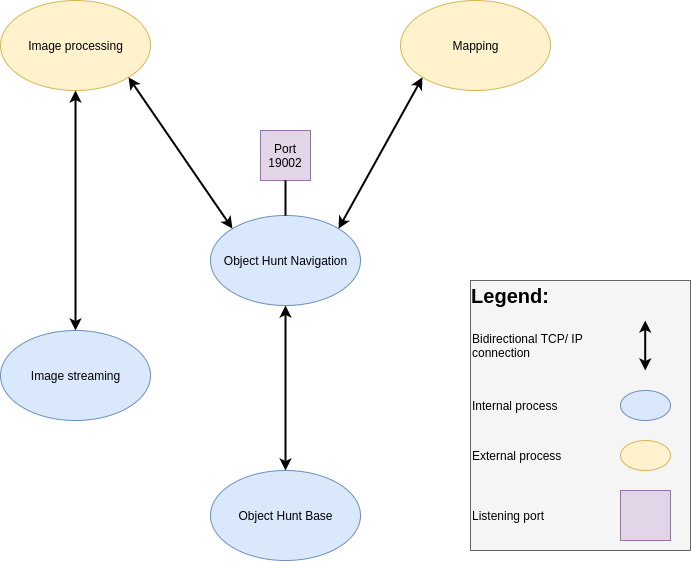
\includegraphics[scale=0.6]{sources/software_structure.png}
\caption[Software structure]{Software structure}
\label{fig:software}
\end{figure}

\subsection{Design Principles}

The system in its entirety shall not be bound to any programming language. In that way virtually any language that supports the usage of raw sockets in collaboration with TCP/\,IP can be used to develop software for the system. At the time of writing this report Java, Python and C++ are already employed.\\

Furthermore underlies the internal software particular specifications, which are defined at the beginning of the project. They define, among other things, how the system as a whole will behave and handle dedicated tasks, i.e. inter-process communication. The compliance of these principles ensure that the developed software works in the expected manner and offers the possibility for adding further processes in the future.\\

The defined principles are listed in the following:

The internal software underlies software specifications, which are defined at the beginning of the project. They define among other things how the system as a whole will behave and handle dedicated tasks, i.e. communication. The compliance of these principles ensure that the developed software works in the expected manner and offers the possibility for adding further processes in the future.


\begin{itemize}
\itemsep0em
\item Communication
	\begin{itemize}
	\item Via TCP/\,IP
	\item Independent from other devices
	\item Beyond system border
	\end{itemize}
	
\item Economical
	\begin{itemize}
	\item No unnecessary CPU consume
	\item Fast reaction times
	\item Event driven
	\end{itemize}
	
\item Documentation
	\begin{itemize}
	\item Complete
	\item Easy accessible
	\end{itemize}
\end{itemize}

\subsubsection{Communication}

All participating processes communicate via TCP/\,IP. Therefore a purpose-built way of exchanging data is developed. Messages are generally separated in action identifiers, commands, requests and responses. Table \ref{tbl:message_definition} declares the usage of each message type.

\begingroup
\begin{tabular}[t]{|l|l|}
\hline
\makecell{Action\\identifiers} & \makecell{This messages consist of exactly one byte in all implementations. It is put in front of\\each other message type and tells the receiving process what data is about to come in.}\\
\hline
Commands & \makecell{Gives a specific order to the base process. Only the base process can handle commands.\\A command does not implicate any result, so the sending process will get no feedback,\\if the command succeeded or not.}\\
\hline
Requests & \makecell{Asks for the cars state. That can be in particular a reading of one or several sensors,\\speed or orientation data. Every request implicates a response with the desired value.\\Each request contains an identifier field.}\\
\hline
Responses & \makecell{A response message will always follow an earlier request. It can either\\indicate an invalid request or contain the desired data. Each response contains an\\identifier field. It will adopt the identifier of the respecting request.}\\
\hline
\end{tabular}
\captionof{table}{Definition of messages}\label{tbl:message_definition}
\endgroup

There exist several implementations of each message type. A motor will most likely be controlled by a respecting command message. A sensor measurement on the other hand can be triggered by a correct request. Please refer to the project documentation page \cite{docu} for further information about which messages exist and their exact composition.

\subsubsection{Economical}

The application shall be both CPU as well as time efficient. Therefore the participating processes are implemented in a multi-threaded manner. Each thread gets created at initiation and is dedicated to one task. A thread will only be active, if the respecting task needs to executed. Otherwise the thread will be in an idle and consume no unnecessary CPU time. Tasks are getting triggered by certain events, i.e. a hardware interrupt, an incoming message, an expired timer and so on. All events are initialized so that they can get polled from file descriptors. This allows threads and processes to wait in an idle state for specific events to happen.\\

In a multi threaded context one has to take care of simultaneous access of shared resources. Therefore the threads are synchronized via synchronization mechanisms, for example mutexes. A mutex can be shared between multiple threads. If one of the threads needs to access a shared resource, it will lock the mutex. When another thread tries to access the same resource in the same time, it would need to lock the mutex as well. When the mutex is locked already, the calling thread is queued until the mutex is unlocked. As soon as the mutex gets unlocked by the initial thread, the queued thread will lock it and access the resource. In this work exclusively scoped locks are used. A scoped lock gets created whenever a mutex shall be locked. The respecting mutex is passed to the constructor of the scoped lock. The scoped object will be destroyed when its scope is left and releases the mutex. This prevents a so called deadlock situation, in which a mutex is locked and cannot be unlocked anymore. A possible scenario for this is, if the locking thread experiences an error and get stopped before unlocking the mutex.\\

The communication between different threads is realized through pipes. A pipe offers a writing as well as a reading end. Thus it allows simultaneous writing and reading by two threads without additional synchronization mechanisms. The inter-thread communication is mainly used to exchange information, abort running tasks and notify each other about particular events.

\subsubsection{Documentation}

A complete and accurate documentation of the source code is produced. The software documentation tool Doxygen \cite{doxygen} is used to generate valid HTML\footnote{Hypertext Markup Language (HTML) is the standard markup language for documents designed to be displayed in a web browser} documents from annotated header files. Doxygen creates HTML files, which are displaying the relations between various programming structures (classes, namespaces, ...). Besides developers can add special denoted comments with explanatory content that are going to be adopted in the HTML files. Additional several auxiliary HTML pages with explanatory context regarding the project are created and linked to the pages created by doxygen. All created pages \cite{docu} are public accessible via the internet.\\

Moreover a Github repository \cite{github} is arranged. It contains the source code, mechanical construction files, schematics, PCB files, the documentation and so forth. The data contained in the Github repository allows to rebuild the whole system developed in this work from scratch. 

\subsection{Base Process}

The base process interacts directly with all controllable hardware parts listed in section \ref{sec:hardware}. Therefore it is a crucial process for the correct function of the robot. If the base process crashes unexpected, any other process concluded in the project will be disconnected or shut down as well.\\

\subsection{Navigation Process}



\newpage

\section{Image Processing}\label{sec:image_processing}

\subsubsection{Definition of the object detection task}

In the deep learning computer vision area are different tasks, which serve different purposes. In figure \ref{fig:object_detection} we can the see the representation of these different tasks. In our project we will take a closer look on the object detection. Like we can see in the image, object detection is capable of detecting multiple objects. But the task is not only to detect and classify them, it is also the task of the program to locate the objects. This will be evaluated on the bounding box around the object.  The desired result can be seen in the following figure.

\begin{figure}[H]
\centering
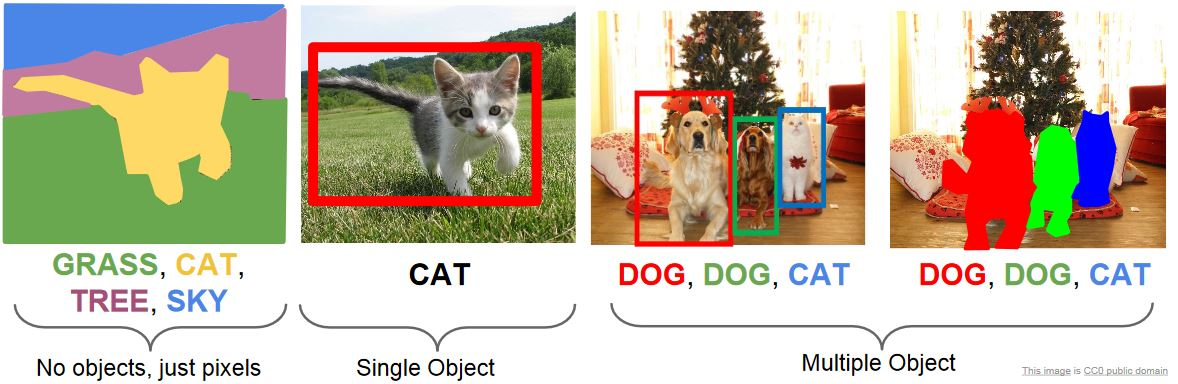
\includegraphics[width=\textwidth]{sources/object_detection.png}
\caption[Image processing task]{Representation of image processing tasks}
\label{fig:object_detection}
\end{figure}

\subsubsection{Requirements on object detection}

In our project we only define the object, which we want to detect. It is not defined how many of these objects will be present, but for the expandability of the project, we will use methods capable of detecting multiple objects.\\

Also the image processing needs to be real-time capable. The roboter navigates autonomously around an unknown area and should detect the objects, when they appear. It is not desirable to have delays in the detection. For this also a sufficient accuracy is needed to detect the object under different lighting and background conditions. \\

So it is a valid trade-off to give up some accuracy for having real-time capability

\subsection{Basic model selection}

Regarding this requirements, we need a specialized model to match the real-time capabilities, while having a decent accuracy. In the image recognition area, the drive for increasing accuracy leads the progress. But it comes with the cost of increasing complexity of the models. This leads to increasing computational cost, which decrease the real-time capabilities. Mobile phones and embedded system are not capable of providing this performance. For this purpose the MobileNet \cite{tim1} network was created. It drastically decreases the number of trainable parameters with different techniques. The main difference from conventional networks is the depthwise convolution. In the conventional convolutional networks the convolution determines features by applying kernel filters on the different input channels and combines the features to reach a new representation \cite{tim1}\\

This results in a computational cost of:

$$ D_K \cdot D_K \cdot M \cdot N \cdot D_F \cdot D_F$$

The MobileNet splits these two steps up and computes them seperatly \cite{tim2,tim3}.  First the depthwise convolution is applied by applying a single filter per input channel. In the second step the pointwise convolution combines the resulting features. Both of these operations present an own layer and are followed by a batch normalization and a ReLU activation. This separation results in a new computational cost of:

$$ D_K \cdot D_K \cdot M \cdot D_F \cdot + M \cdot N \cdot D_F \cdot D_F $$

Comparing these to costs, the depthwise convolution reaches a reduction of $ \dfrac{1}{N} + \dfrac{1}{D^2_K} $.

\begin{figure}[H]
\centering
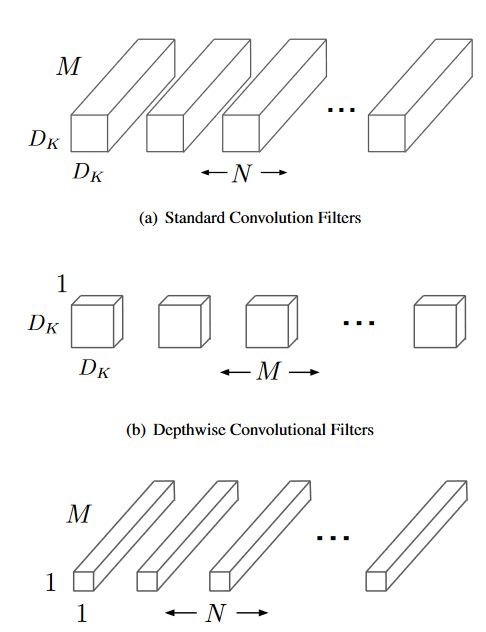
\includegraphics[scale=0.65]{sources/depthwise_convolution.JPG}
\caption[Comparison standard and depthwise]{Comparison of standard convolution (a) and Depthwise Convolution \cite{tim2,tim3}}
\label{fig:depthwise_convolution}
\end{figure}

The Mobile network was tested one time with standard convolution and with depthwise separable convolution. The result was only 1,1\% loss in accuracy, but a reduction of 25,1 million parameters. 

\begin{figure}[H]
\centering
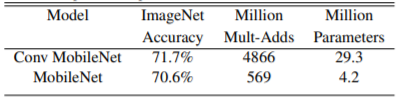
\includegraphics{sources/Comparison_Mobilenet.png}
\caption[Comparison standard and separable depthwise]{Comparison of standard and depthwise separable convolution}
\label{fig:depthwise_convolution}
\end{figure}

\section{Object Detection System}

For the object detection there are mainly three different techniques, which are used.

\subsubsection{Faster R-CNN}

One approach is the Faster R-CNN, which is the combination of two modules. First we have a deep convolutional network, which extracts the features. After this the feature map will be shared with a separate network, which predicts the region proposals. In this RPN module the feature map will be fed into two fully-connected layers. One layer computes the box regression and the other one computes the box classification. These predictions will be reshaped through a RoI (Region of Interest) pooling layer and will then be used to classify the found objects within the proposed regions.

\begin{figure}[H]
\centering
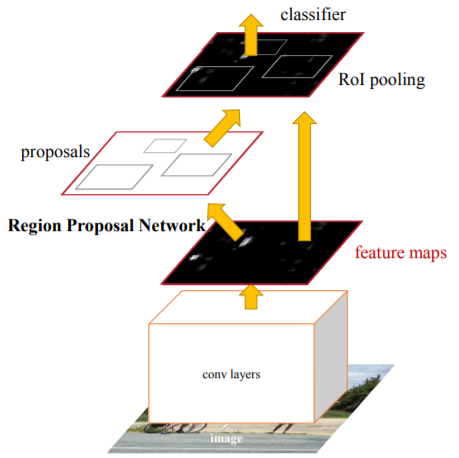
\includegraphics{sources/Faster_R-CNN.png}
\caption[Architecture of Faster R-CNN]{Architecture of Faster R-CNN \cite{tim2}}
\label{fig:depthwise_convolution}
\end{figure}

\subsubsection{You Only Look Once -- YOLO}

Another approach is to not look at regions with high probability of containing an object, but to split the whole image into a grid and predict first the class probability and secondly the offset for the bounding box for different bounding boxes in this grid. The only probabilities higher than a defined threshold will be taken into consideration. This reduces the architecture to one network and eliminates the bottleneck separate classification and bounding box regression. This approach is called YOLO (You Only Look Once), which is a lot faster than Faster R-CNN, but has the drawback of less accuracy \cite{tim3}.

\subsubsection{Single Shot Detection -- SSD}

The last approach uses the same technique as YOLO, but has some diversifications. Single Shot Detection (SSD) is also a one-stage detection model. It predicts class and bounding box at the same time. Unlike YOLO it will not predict the certainty of the object being an object, its only predicts the class probabilities, but adds a background class. So when the background class has a high probability, it has the same effect as a low confidence score from the YOLO prediction.\\

Also the SSD uses different grid layouts, which results in more predictions, but also in more accuracy. Therefore the YOLO architecture delivers better real-time capabilities, because is it less computational intense.

\begin{figure}[H]
\centering
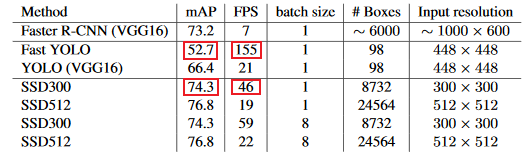
\includegraphics{sources/tempsnip.png}
\caption[Performance comparison of different techniques]{Performance comparison of different techniques \cite{tim5}}
\label{fig:depthwise_convolution}
\end{figure}

\subsection{Experiments}

For our object detection experiments we used the following software components:

\begin{itemize}
\itemsep0em
\item Python 3.7.3
\item OpenCV 4.1.2 \cite{tim6}
\item ImageZMQ \cite{tim7}
\item Imutils \cite{tim8}
\item ssd\_mobilenet\_v2\_coco \cite{tim9}
\end{itemize}

We used OpenCV, because it is a well-established computer vision library and designed for fast computation also on system with low computational capabilities. It offers the DNN (Deep Neural Network) module, which offers methods to import pretrained models from different frameworks. We decided to take the pretrained MobilenetV2 in combination with SSD trained on the COCO dataset. For reasons shown in Section Basic model selection and object detection, we decided this network will give us enough computation speed to detect object while driving and sufficient accuracy to detect the object in different lighting or environment conditions. The COCO (Common Objects in Context) dataset is a commonly used dataset and offers a lot of classes. We defined the Sports ball class as the desired object to detect but wanted to have flexibility to change the object if needed. Therefore, the COCO dataset was well-suited for our requirements.\\

The ``ImageZMQ'' package is a little library with methods to transport the OpenCV images over the network. It uses the ZeroMQ sockets to enable an easy and fast transport.\\

The ``imutils'' package is used to build up the presentation of the images.

\subsection{Software}

Because The images will be sent over network to an external device, two scripts will be started. One is the client script, which runs on the Raspberry Pi. The server script runs on the external device and receives and processes the images. It also sends the acknowledgement to signal the client to send another picture.

\begin{figure}[H]
\centering
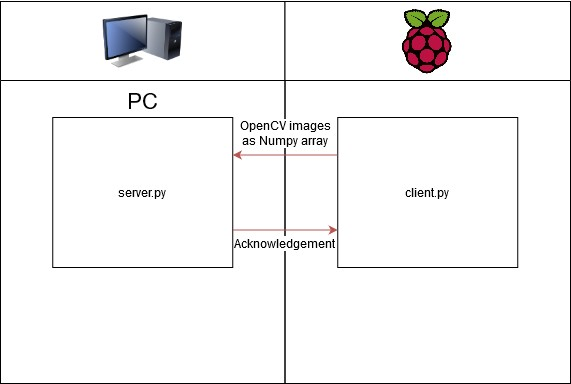
\includegraphics[scale=0.8]{sources/client_server.jpg}
\caption[Server client communication]{Server client communication}
\label{fig:depthwise_convolution}
\end{figure}

\subsubsection{Server.py}

The server first initializes the socket to receive the images and the connection to the ``Object\_hunt\_base'' process. Then the network will be initialized and the objects to consider.\\

The marker for a found object will be set to False before the loop. In the loop the image will be received if there is a connection. If the device is not already known, it will be added to the ``lastActive'' list. The image will be resized and then processed by the network.  If an detection of the desired object occurred and the confidence is higher than the defined threshold, the presentation will be build. The bounding box will be added to the picture and the number of detected objects will be updated. This image will then be shown on the external device. The loop is also interrupted and the connection to the object\_hunt\_base process will be established to send the message of successful object detection. Then the picture of detection will be shown, until the user interrupts the script.

\subsubsection{Client.py}

The client initializes the connection to the server and also initialized the camera. Then in an endless loop it will send the images to the server.

\subsection{Results}

We could realize all the requirements we set for our object detection taks. Our project has shown, that for real-time object detection it is possible to let the image processing run on an external device and still get sufficient results. Our object detection is flexible in detecting different classes, it is possible to choose one of all COCO classes. To get better accuracy and better performance an own dataset will be needed. With this dataset, the network would only predict two different classes, the background and the desired object, which result in much less predictions and therefore better performance.

\newpage

\section{Routing \& Mapping}

A further part of the vehicle is to log the driven route and build a map by detecting the environment.
As shown in figure \ref{route_map} the vehicle drives autonomous threw an unknown environment. During the
ride all objects besides the vehicle will be detected by sensor. The driven route will be logged by
storing the events of drive like orientation changes.\\
\begin{center}
\begin{minipage}{0.45\textwidth}
\label{route_map}
\includegraphics[page=3,scale=1]{sources/mapping/example_tunnel.pdf}
\captionof{figure}{Routing \& Mapping}
\end{minipage}
\end{center}

\subsection{Detection}

\subsubsection{Routing}

\begin{minipage}{0.5\textwidth}
By the installed hardware it is possible to measure the current orientation (angle) and the current speed. These values can be used to calculate the movements of the vehicle.\\
At the start of the processes and the vehicle an initialization will be proceeded, which sets the current position on an imaginary coordinate system at the point (the coordinates) (0,0)[x,y]. From this point the movements of the vehicle will be logged by calculating every new position respectively coordinate in a list.
\end{minipage}
\begin{minipage}{0.5\textwidth}
\centering
	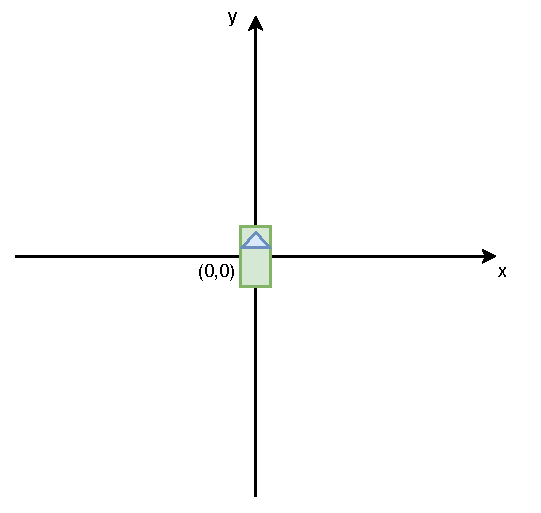
\includegraphics[scale=0.6]{sources/mapping/initial_position.pdf}
	\captionof{figure}{Initial position}
\end{minipage}

\begin{minipage}{0.5\textwidth}
\centering
	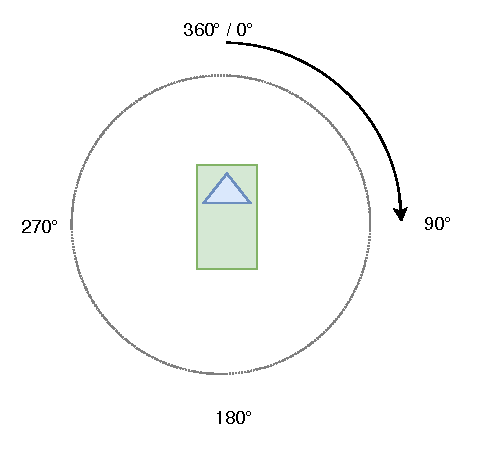
\includegraphics[scale=0.6]{sources/mapping/orientation.pdf}
	\captionof{figure}{Vehicle orientation}
\end{minipage}
\begin{minipage}{0.5\textwidth}

By using the smart movement sensor the orientation respectively the angle of the vehicle can measured, in relation to the initial position / orientation which is 0\degree.

By using the smart movement sensor the orientation respectively the angle of the vehicle can measured, in relation to the initial position / orientation which is 0\degree.

\end{minipage}

\begin{minipage}{0.5\textwidth}
The vehicle provides an revolution sensor by which one the current speed $v$ of the vehicle can be measured. Every time the speed changes the cuttent time will be stored. With speed $v$ and the time slot $t$ the driven distance $s$ during this time slot can be calculated by $s=\frac{v}{t}$.
\end{minipage}
\begin{minipage}{0.5\textwidth}
	\centering
	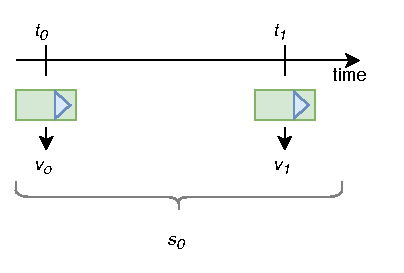
\includegraphics[scale=0.8]{sources/mapping/distance.pdf}
	\captionof{figure}{Calculated driven distance}
\end{minipage}
\\
\\
By the resulting driven distance and the orientation of the vehicle the coordinates (related to the initial position and the following positions) can be calculated. The order of these coordinates results in the driven route.

\begin{minipage}{\textwidth}
	\centering
	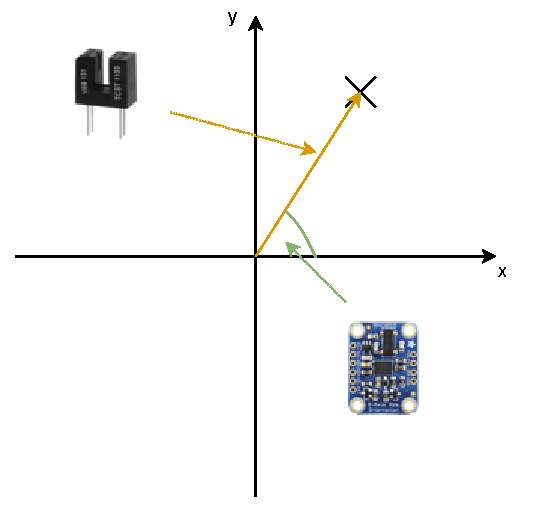
\includegraphics[scale=0.6]{sources/mapping/orientation_distance.pdf}
	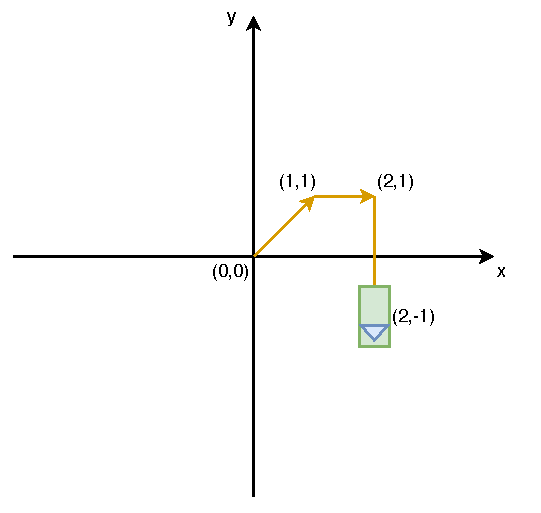
\includegraphics[scale=0.6]{sources/mapping/route.pdf}
	\captionof{figure}{Logged route information}
\end{minipage}
\\
\\
By the information of the driven route the current position of the vehicle is known.



\subsubsection{Mapping}

To detect object around the vehicle respectively the environment ultra sonic sensors are used. On the vehicle four sensors are installed, one at the front, rear, left and right.\\
The detected objects will be also logged by coordinates in relation to the current position and orientation of the vehicle.\\
In the beginning the sensor data will be read. These data will stored in coordinates which will adjust by adding the orientation of the vehicle to calculations. Finally, the calculated coordinates will be added to the current position coordinates of the vehicle to result the object position in relation to the initial point (0,0).

\begin{center}
	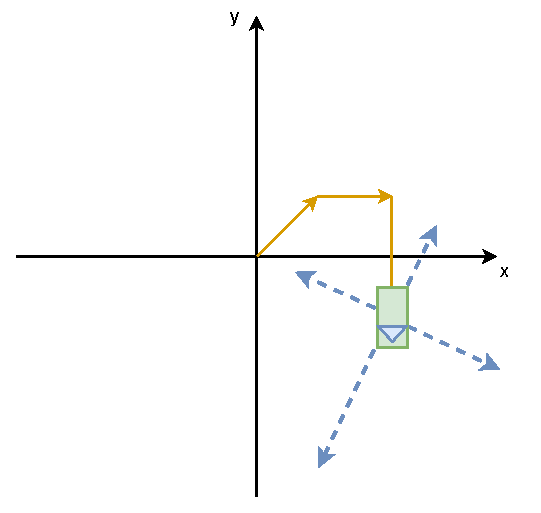
\includegraphics[page=1,scale=0.6]{sources/mapping/orientation_objectdistance.pdf}
	\includegraphics[page=2,scale=0.6]{sources/mapping/orientation_objectdistance.pdf}
	\includegraphics[page=3,scale=0.6]{sources/mapping/orientation_objectdistance.pdf}
	\captionof{figure}{Smart movement and ultra sonic sensor}
\end{center}

\newpage

\subsection{Software}

The routing \& mapping progress is a self-contained process as described in the beginning of this report and has been developed with Java.\\
\\
It contains several classes which will be show following:

\begin{table}[h]
\begin{center}
	\begin{tabular}{|p{0.3\textwidth}|p{0.7\textwidth}|}
		\hline
		Class & Description\\\hline\hline
		ProcessMain & Includes the main-methode to start the process by calling the method \textit{processControl()} of the class ProcessControl. It also may be used call additional method of further classes which may be added.\\\hline
		ProcessControl & Calls the relevant methods to run the important tasks.\\\hline
		SystemData & Stores the system relevant information like port or communication codes.\\\hline
		NetworkInterface & Establishes the network communication with the navigation process.\\\hline
		LogFile & Creates and edits the log files.\\\hline
		MessageAnalysis & Checks the received messages and their contents and handles the following processing\\\hline
		MapData & Stores and handles the data for the route and map building.\\\hline
		Calculations & Offers the methods for the calculations.\\\hline
		DrawRoute & Includes the methods for the route.png to be created.\\\hline
		DrawMap & Includes the methods for the map.png to be created.\\\hline
	\end{tabular}
	\caption{Process classes}
	\end{center}
\end{table}


As described before the relevant methods for this process will be called by the method \textit{processControl()}, which is shown below. To describe this the sequence more understandably the program sequence is graphically shown in figure \ref{programSequence}

\lstset{language=Java,
   basicstyle=\small,
   keywordstyle=\color{blue!80!black!100},
   identifierstyle=,
   commentstyle=\color{green!50!black!100},
   stringstyle=\ttfamily,
   breaklines=true,
   numbers=left,
   numberstyle=\small,
   frame=single,
   backgroundcolor=\color{blue!3}
}
\lstset{language=Java}

\begin{lstlisting}
public void processControl() {
	processInitialisation();
	while(!system.endOfProcess) {
		analysis.checkMessage(network.readSocket());
	}
	System.out.println("\nBuilding route...");
	drawRoute.buildMap(mapData.routeX, mapData.routeY, "Route", routeCoordinates);
	System.out.println("route.png created.\nBuilding map...");
	drawMap.buildMap(mapData.mapX, mapData.mapY, "Map", mapCoordinates);
	System.out.println("map.png created.\n");
		
	System.out.println("System ends.");
}
\end{lstlisting}
\captionof{lstlisting}{Method \textit{processControl()}}

In the beginning an initialization process will be proceeded. This includes the establishment of the network communication with the navigation process. Also, the first data of the sensor will be received to initialize the start position of the vehicle and respectively the center of the coordinate system (0,0).\\


\begin{minipage}{0.4\textwidth}
The code of the process includes a boolean variable which will be set true if the navigation process wants the process to be ended. This variable will check every time the while-loop start at the beginning. After this check the process wait for a message to be received in depend on the type of information to be received.\\
There are two options of informations to be received. The message could have the length of one byte, then this byte gives informations if the process has to stop, the vehicle rotates or which type of values will be send in the message. With that type of information the knows the byte array length of the next message. \\
If the message is longer than one byte the message includes sensor data and can be directly transfer to the methods which handle value data.\\
\end{minipage}
\begin{minipage}{0.6\textwidth}
\label{programSequence}
\begin{center}
	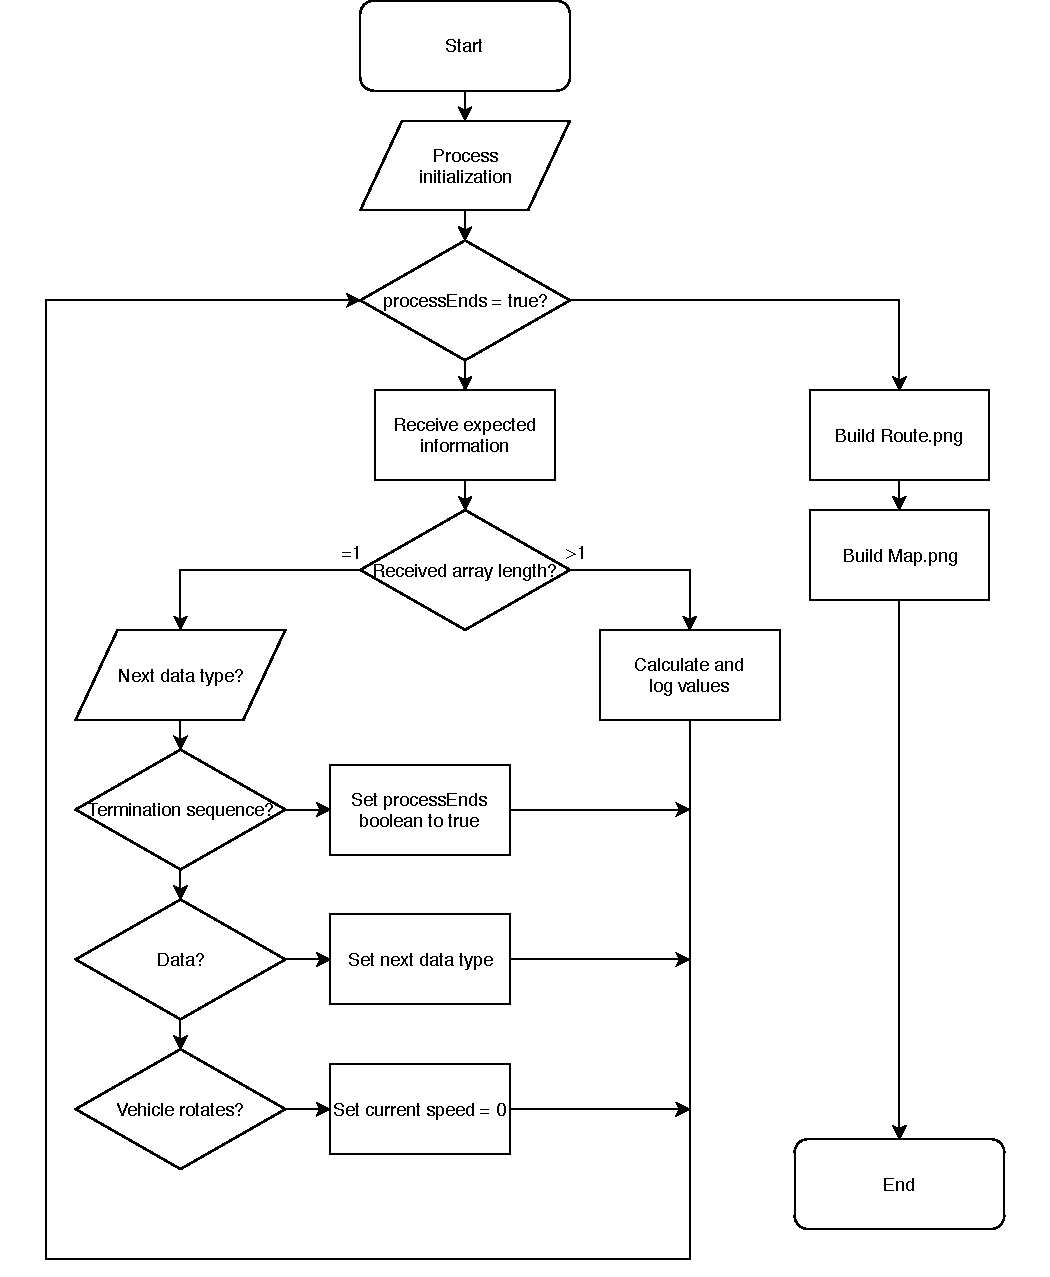
\includegraphics[scale=0.6]{sources/mapping/program_sequence.pdf}
	\captionof{figure}{Program sequence}
\end{center}
\end{minipage}

Finally the while-loop start at the beginning till the navigation process sends the termination sequence.\\
If this sequence will be received the while-loop stops and the methods to build the grphicals files for the route and the map will be called.

\begin{center}
	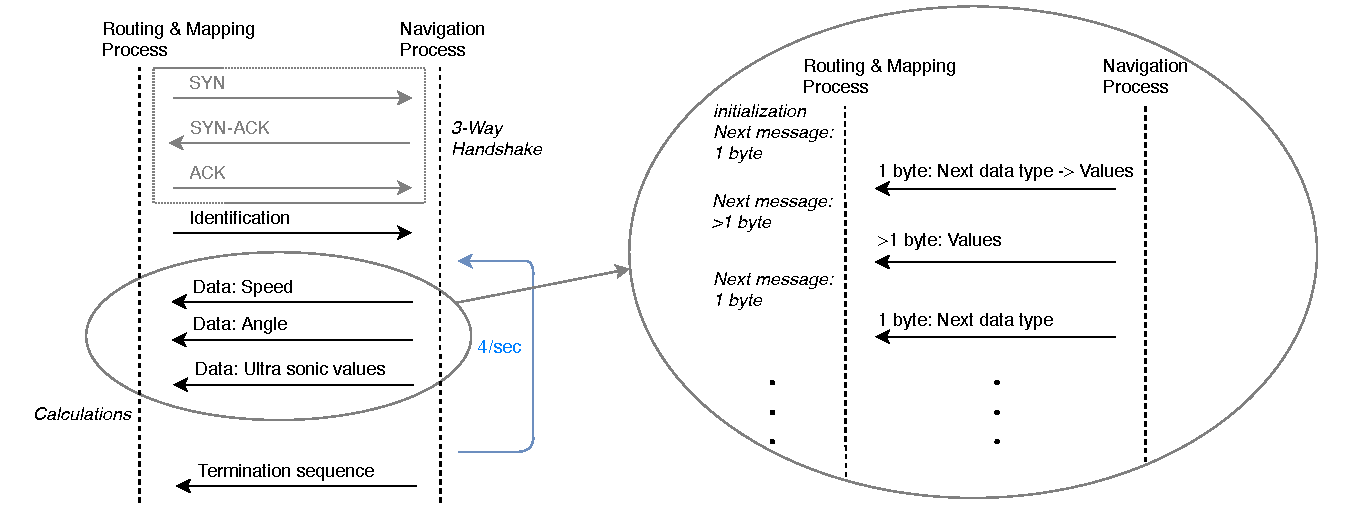
\includegraphics[scale=0.7]{sources/mapping/communication.pdf}
	\captionof{figure}{Principle commuication}
\end{center}


During the process run all the calculated coordinates of the route and the map respectively the objects will be stored in log files. At the end of the process the classes DrawRoute and DrawMap read the named files to get the coordinates. By these coordinates the wanted .png files will be created as shown below.

\begin{minipage}{0.5\textwidth}
\begin{center}
	\includegraphics[scale=0.015]{sources/mapping/Route.png}
	\captionof{figure}{Route.png}
\end{center}
\end{minipage}
\begin{minipage}{0.5\textwidth}
\begin{center}
	\includegraphics[scale=0.015]{sources/mapping/Map.png}
	\captionof{figure}{Map.png}
\end{center}
\end{minipage}


\subsection{Problems}

Unfortunately some problems with the ultra sonic sensors occurred.\\
The measured distance of the objects are not continuously correct respectively useful. By this error it is not possible to build an adequate map. The main object which are visible in the map build the shape of the route. The object in which direction the vehicle drives will be detected several times but with kind of random values. This causes the visible shape of the route in the map.
\newpage

\section{References}
\begin{flushleft}
\begin{thebibliography}{99}
\bibitem[1]{l293dne} Texas Instruments Incorporated, ``L293x Quadruple Half - H Drivers -- Data Sheet'' 2016 [Online]. Available: \url{https://www.ti.com/lit/ds/symlink/l293d.pdf}. [Accessed: 31.01.2020].
\bibitem[2]{tcst1103} Vishay Semiconductors, ``Transmissive Optical Sensor with Phototransistor Output'' 2011 [Online]. Available: \url{https://www.vishay.com/docs/83764/tcst1103.pdf}. [Accessed: 31.01.2020].
\bibitem[3]{hc_sr04} Elec Freaks, ``Ultrasonic Ranging Module HC - SR04'' [Online]. Available: \url{https://cdn.sparkfun.com/datasheets/Sensors/Proximity/HCSR04.pdf}. [Accessed: 31.01.2020].
\bibitem[4]{bno055} Adafruit, ``BNO055 Absolute Orientation Sensor'' 2015 [Online]. Available: \url{https://learn.adafruit.com/adafruit-bno055-absolute-orientation-sensor/overview}. [Accessed: 31.01.2020].
\bibitem[5]{rpi4} Raspberry Pi foundation, ``Raspberry Pi 4 Model B'' [Online]. Available: \url{https://www.raspberrypi.org/products/raspberry-pi-4-model-b/}. [Accessed: 31.01.2020].
\bibitem[6]{eagle} Autodesk, ``EAGLE overview'' [Online]. Available: \url{https://www.autodesk.com/products/eagle/overview}. [Accessed: 31.01.1020]. 
\end{thebibliography} 

\end{flushleft}



\end{document}